\documentclass{article}
\setlength{\oddsidemargin}{0.25 in}
\setlength{\evensidemargin}{-0.25 in}
\setlength{\topmargin}{-0.6 in}
\setlength{\textwidth}{6.5 in}
\setlength{\textheight}{8.5 in}
\setlength{\headsep}{0.75 in}
\setlength{\parindent}{0 in}
\setlength{\parskip}{0.1 in}

% ===== PACKAGES =====
\usepackage{amsmath,amssymb}
\usepackage{color}
\usepackage{subfigure}
\usepackage{mdframed}
\usepackage{changepage}
\usepackage{graphicx, hyperref}
\newmdenv[
  topline=false,
  bottomline=false,
  skipabove=\topsep,
  skipbelow=\topsep
]{siderules}
\renewcommand{\abstractname}{}

% ===== VARIABLES =====
\def \R{\mathbb{R}}
\def \Pr{\mathbb{P}}
\def \D{{\rm D}}
\def \N{{\rm N}}
\def \xx{{\boldsymbol{\rm x}}}
\def \y{{\rm y}}




% ===== HEADER BOX =====
\newcommand{\lecture}[2]{
\pagestyle{myheadings}
\thispagestyle{plain}
\newpage
\noindent
\begin{center}
\rule{\textwidth}{1.6pt}\vspace*{-\baselineskip}\vspace*{2pt} % Thick horizontal line
\rule{\textwidth}{0.4pt}\\[1\baselineskip] % Thin horizontal line
\vbox{\vspace{2mm}
\hbox to 6.28in { {\bf CS 760: Machine Learning} \hfill Fall 2020 }
\vspace{4mm}
\hbox to 6.28in { {\Large \hfill #1  \hfill} }
\vspace{4mm}
\hbox to 6.28in { {\scshape Authors:}  #2 \hfill }}
\vspace{-2mm}
\rule{\textwidth}{0.4pt}\vspace*{-\baselineskip}\vspace{3.2pt} % Thin horizontal line
\rule{\textwidth}{1.6pt}\\[\baselineskip] % Thick horizontal line
\end{center}
\vspace*{4mm}
}



% ===== GRAPHICS PATH =====
\graphicspath{
	{../pics/}
}



% =============== DOCUMENT ===============
\begin{document}
\lecture{Predicting COVID-19 Hospitalizations of Mexican Indigenous People}{Edwin Baeza}

\begin{center}
{\Large {\sf GO GREEN. AVOID PRINTING, OR PRINT 2-SIDED OR MULTIPAGE.}}
\end{center}

\begin{abstract}
Our aim for this project was to construct models to predict the hospitalization of an indigenous person due to Covid-19. We employed decision trees including random forests, and logistic regression. After analyzing precision-recall curves and cross validating, we find that our models fail to provide sufficient precision to be deployable.      

 

\end{abstract}

\section{Introduction}
The COVID-19 pandemic is raging across North America and exacerbating the challenges some of the most vulnerable populations face. One such example are the indigenous people of Mexico. In 2018, an estimated 80.6\% of the indigenous population in Mexico are considered to be extremely poor while only accounting for 12.6\% of the wider population. Often residing in rural areas where there may be little or no access to conventional health services, many indigenous people turn to \emph{curanderos} (local healers/shamans) \cite{un}.     

Our goal for this project was to construct machine learning models that predict whether an indigenous person that tested positive for COVID-19 in Mexico would end up in the ICU. Our motivation was to help indigenous communities and those that serve them make informed decisions regarding the distribution of  resources for those that contract COVID-19. A successful model would, for instance, allow communities to identify those who are at a higher risk for hospitalization and, hopefully, provide a buffer so these communities can gather funds/resources should these individuals need to be hospitalized.      


\section{Related/Similar Work}
Of course, there are analyses of COVID-19 in Mexico and some also focus on indigenous people. For example, statistical methods are employed in \cite{survival_analysis} and \cite{demo_comorbid}. Statistics also seems to be the focus of \cite{impact}, which was similar in spirit to goal. A machine learning approach is taken in  \cite{predictive_models}, but their focus is on the Mexican population as a whole. To the best of our knowledge, this may be the one of the first attempts to build such predictive models for indigenous people.   


\section{Dataset}
The raw data was obtained from the Mexican Ministry of Health (Secretaría de Salud, SS) through the Epidemiological Surveillance System for Viral Respiratory Diseases \cite{gob_mex}. For our analysis we used the data as of December 2, 2020. 

The raw data consisted of two Excel files, a CSV file, and a pdf. These files were further split into two folders, 
diccionario\_datos\_covid19 and datos\_abiertos\_covid19. The first folder contained the Excel and pdf files: the raw data descriptors (201128 Descriptores\_), the raw data categories (201128 Catalogos), and a pdf describing changes made to the data (Actualizaciones en la presentación de información referente a casos de COVID). We referenced these files to aid in feature selection. The second folder contained csv data with information recorded on every individual related to COVID-19. The information recorded includes: sex, age, nationality, place of residence, ICU, indigenous, speak indigenous language, chronic diseases, immuno-suppression, other diseases reported by the individual, pregnancy, and smoking. The raw data here contained 2919879 rows and 40 columns. 

The next step was to preprocess the raw data with pandas and a Juptyer notebook. Our first step was to selected the features most relevant to our goal. For example, the raw data included categories for whether an individual identified as indigenous or spoke an indigenous language. For simplicity, we chose to only look at individuals that identified as indigenous. There were also different classes for COVID-19 testing, but, again, we took only individuals with a confirmed positive test for simplicity and also for specificity.  

After using the above two features to filter the data, we chose the remaining physiological features. The final features selected were: Sex, Age, Pregnancy, Pneumonia, Diabetes, COPD (Chronic Obstructive Pulmonary Disorder), Asthma, Immunosuppresion, Hypertension, Other Conditions, Cardiovascular, Obesity, Chronic Kidney Disease, Smoking, and ICU. Except for Age, all these features in the raw data are primarily binary with values 1 or 2 (and other values for not applicable/to ignore/ not specified). For simplicity, we convert the features into binary 1 and 0. As a result, we reduced the raw data to 11433 rows × 15 columns. 

The data we will pass on is described mathematically as follows: a feature vector is represented by $x$, our response is a binary variable $y$, we we have $D = 14$ features (almost all of which are binary), and $N = 11433$ feature vectors.

    
\section{Approach}
The packages/libraries we used are pandas, matplotlib, and sklearn. We will elaborate on their use below.  We run all of our code on Jupyter notebooks. 

We note that in the processed dataset there are only 338 individuals in the ICU. Being hospitalized is a rare event, so our data is imbalanced. To address this somewhat, we split our data into train/test sets utilizing the \emph{train\_test\_split} method from the \emph{sklearn.model\_selection} package. We are able to reserve 25\% of the processed data for testing, fix the random state for reproducibility, and set the splitting to be stratified. Stratifying is important here, as the data is imbalanced. We recall that stratifying splits our data while maintaining the relative frequency of each class, in this case ICU and Not ICU. By stratifying, we ensure that our model predictions are not inflated by choosing ICU most of the time.      

The algorithms we decided to use were decision trees, random forests, and logistic regression. We chose these algorithms because their simplicity in implementation works well as a starting point. We will elaborate on each of these algorithms below. 

For our decision tree we used the \emph{DecisionTreeClassifier} method from \emph{sklearn.tree} package. The criterion for splitting was information gain (``entropy" in the method declaration). We set the max depth of the tree to be 5. This depth was chosen as it maximized average precision, see the results below. Since our data is imbalanced, to improve algorithm performance, we set the \emph{class\_weight} parameter to ``balanced". This parameter ensures that the algorithm uses the values of $y$ to automatically adjust weights inversely proportional to class frequencies in the input data. The other parameters are left as defaults.                                 

For our random forest we used the \emph{RandomForestClassifier} method from \emph{sklearn.ensemble} package. The number of trees in our forest was set to 100, the default value. The criterion for splitting was again information gain, just as for the decision tree. We similarly set max depth to 5 and the \emph{class\_weight} parameter to ``balanced".

For logistic regression we used the \emph{LogisticRegression} method from \emph{sklearn.linear\_model} package. The \emph{class\_weight} parameter to was set to "balanced" and the \emph{solver} parameter was set to ``newton-cg". This parameter tells the method to use the newton conjugate gradient method to optimize.    

Our algorithms were evaluated using 10-fold cross-validation. The metrics we kept track were accuracy, recall and precision. Of these, precision is the most important, since we are trying to predict a rare event. We note that accuracy here can be misleading, since we can inflate it just by simply labeling everything as Not ICU. We will visualize these metrics with precision-recall curves. Also, we measure each algorithm at specific thresholds for prediction, where each threshold was chosen since it maximized precision.  


\section{Results}
In this section we demonstrate our results and provide a table summarizing them. 

\begin{figure}[h]
\centering
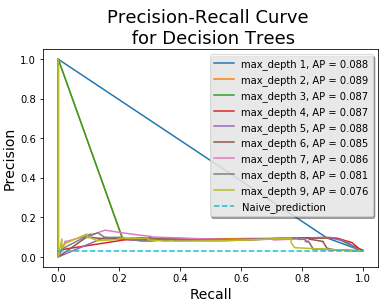
\includegraphics[scale=.9]{DT_Depth_PR_curves}
\caption{Precision-recall curves for decision trees at various depths. }
\label{fig:1}
\end{figure}

Since our data was imbalanced, we used the \emph{predict\_proba} method for each classifier in order to return a probability instead of a label. This allowed us to set a threshold in order to determine a label. To find a suitable thresholds, we plotted precision-recall curves  and recorded their average precision scores. We found that good thresholds provides precision close to this score. Figure \ref{fig:1} shows a glimpse into this process for our decision tree. In Figures \ref{fig:2}, \ref{fig:3}, and \ref{fig:4} we see the precision recall curves for our three algorithms. Figure \ref{fig:5} shows these curves in the same plot. Each algorithm is compared to the baseline naive/no skill algorithm, which just guesses the average number of ones found in the test set.    

\begin{figure}[h] 
\centering
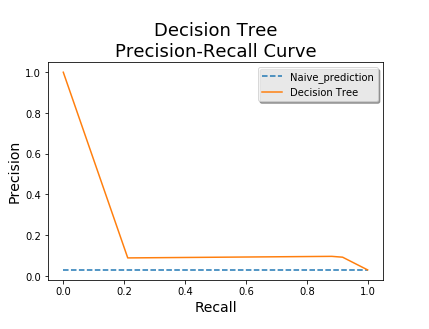
\includegraphics[scale=.9]{DT_PR_curve}

\caption{Precision-recall curve for decision trees}
\label{fig:2}
\end{figure}

 
\begin{figure}[h!]
\centering
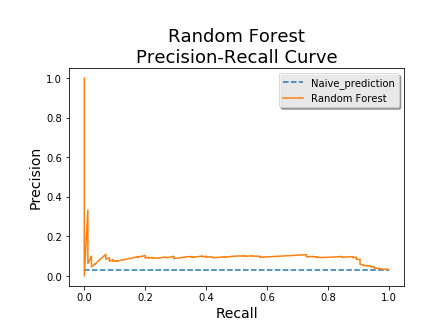
\includegraphics[scale=.9]{RF_PR_curve}
\caption{Precision-recall curve for random forest}
\label{fig:3}
\end{figure}

\newpage

\newpage

\begin{figure}[h]
\centering
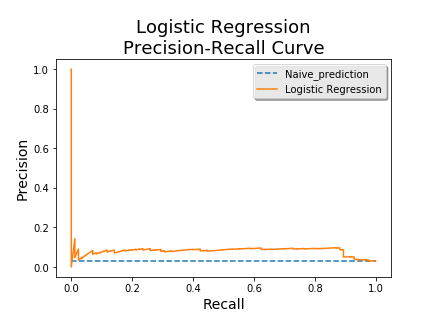
\includegraphics[scale=.9]{LR_PR_curve}

\caption{Precision-recall curve for logistic regression}
\label{fig:4}
\end{figure} 


\begin{figure}[h!]
\centering
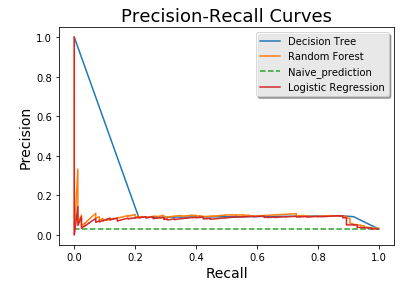
\includegraphics[scale=.9]{ALL_PR_curves}
\caption{Precision-recall curve for our algorithms}
\label{fig:5}
\end{figure}

\newpage
\
\newpage

\begin{figure}[h!]
\begin{tabular}{|c|c|c|c|}
\hline 
 & \textbf{Decision Tree} & \textbf{Random Forest} & \textbf{Logistic Regression} \\ 
\hline 
\textbf{Precision (threshold)} & 0.096 (0.62) & 0.107 (0.62)& 0.097 (0.67) \\ 
\hline 
\textbf{Recall (threshold)} & 0.882 (0.62) & 0.729 (0.62)&  0.871 (0.67)\\ 
\hline 
\textbf{Accuracy (threshold)} & 0.750 (0.62) & 0.811 (0.62) & 0.756 (0.67) \\ 
\hline 
\textbf{10-CV Avg. Precision} & 0.097 & 0.101 & 0.101 \\ 
\hline 
\textbf{10-CV Avg. Recall} & 0.867 & 0.867 & 0.867 \\ 
\hline 
\textbf{10-CV Avg. Accuracy} & 0.749 & 0.761 & 0.760 \\ 
\hline 
\textbf{PR-Curve Avg. Precision} & 0.089  & 0.095 & 0.083 \\ 
\hline 
\end{tabular} 

\caption{Table Summarizing Metric Results }
\label{fig:6}
\end{figure}

\newpage
Finally, below we present a table that summarizes our results. We chose to measure precision, recall, and accuracy of each algorithm at a selected threshold. We also measured the average precision, recall, and accuracy of a 10-fold cross validation. Finally, we measured the average precision of each algorithm's precision-recall curve. 
\newpage


\section{Conclusions and Future Work}
The results are disappointing. All of our models are comparable to each other, as can be seen in Figure \ref{fig:5}, but each one has low precision. The table represents essentially the best that these models can offer. in terms of the raw numbers, it seems that random forest provides the best precision. The recall and accuracy of these models would be acceptable to deploy, but the precision is what really limits the usefulness. 

Different methods of preprocessing could also be used. For example, one could try to one-hot encode the binary variables, but we are not convinced that this would significantly impact any of our models. One could also try to use unsupervised machine learning algorithms, such as principal compnnent analysis or k-means clustering, for better feature selection. This approach has some promise, but may not fully compensate for the data imbalance.          

For future attempts at predictive models, larger dataset could yield better results. Since we are trying to predict a rare event, we imagine that may not be possible. One could supplement the established data via various augmentation techniques such as oversampling the ICU class or generating synthetic ICU data. These should improve the results of our algorithms, but careful analysis is need to ensure the augmented dataset does not obscure relationships in the original data in order to inflate results. 

Similarly, one could undersample the non ICU class to form a diminished dataset. Issues similar to the ones found in data augmentation arise with this technique. Of course, one may try using other algorithms to construct such models. We feel that in the absence of augmented/diminished data, other algorithms would not fare any better that the ones chosen here. 

%\section{References}
\begin{thebibliography}{7}

\bibitem{un} 
State of the World’s Indigenous Peoples, Volume II, Health 
\url{https://www.un.org/development/desa/indigenouspeoples/wp-content/uploads/sites/19/2018/03/The-State-of-The-Worlds-Indigenous-Peoples-WEB.pdf}

\bibitem{survival_analysis} Guillermo Salinas-Escudero, María Fernanda Carrillo-Vega, Víctor Granados-García, Silvia Martínez-Valverde, Filiberto Toledano-Toledano, and Juan Garduño-Espinosa. 
\emph{A survival analysis of COVID-19 in the Mexican population}. BMC Public Health, 2020  

\bibitem{demo_comorbid} Carlos E. Galván-Tejada, Laura A. Zanella-Calzada, Karen E. Villagrana-Bañuelos, Arturo Moreno-Báez, Huizilopoztli Luna-García, Jose María Celaya-Padilla, Jorge Issac Galván-Tejada, and Hamurabi Gamboa-Rosales.
\emph{Demographic and Comorbidities Data Description of Population in Mexico with SARS-CoV-2 InfectedPatients(COVID19): An Online Tool Analysis}. Int J Environ Res Public Health. 2020 Jul

\bibitem{impact} Carlos Medel-Ramírez, and Hilario Medel-López \emph{Impact of (SARS-CoV-2) COVID 19 on the indigenous language-speaking population in Mexico}. 2020 
\url{https://mpra.ub.uni-muenchen.de/102579} 


\bibitem{gob_mex} Government of Mexico. Health Secretary. Databases Covid-19 México.
\url{https://www.gob.mx/salud/documentos/datos-abiertos-152127}.  


\bibitem{predictive_models} Salomón Wollenstein-Betech, Christos G. Cassandras, and Ioannis Ch. Paschalidisa. 
\emph{Personalized predictive models for symptomatic COVID-19 patients using basic preconditions: Hospitalizations, mortality, and the need for an ICU or ventilator}. Int J Med Inform. 2020 Oct.



\end{thebibliography}


\end{document} 

